\documentclass[11pt]{scrartcl}
\usepackage{polski}
\usepackage[polish]{babel}

\usepackage{graphicx, float, caption, subcaption, amsmath}
\usepackage{tabularx, multirow, hyperref, enumitem, listings}
\usepackage{xcolor}
%\usepackage{minted}

\hypersetup{
    colorlinks=true,
    linkcolor=black,
    urlcolor=black,
    citecolor=black
}

\definecolor{md-black}{rgb}{0.12, 0.12, 0.12}
\definecolor{md-teal}{rgb}{0.38, 0.79, 0.69}
\definecolor{md-mauve}{rgb}{0.76, 0.52, 0.75}
\definecolor{md-yellow}{rgb}{0.86, 0.86, 0.67}
\definecolor{md-green}{rgb}{0.13, 0.55, 0.13}
\definecolor{md-red}{rgb}{0.82, 0.10, 0.14}
\definecolor{md-purple}{rgb}{0.69, 0.33, 0.73}
\definecolor{md-orange}{rgb}{0.96, 0.42, 0.18}
\definecolor{md-gray}{rgb}{0.44, 0.46, 0.51}
\lstset{
    language=Python,
    basicstyle=\color{md-teal}\ttfamily,
    keywordstyle=\color{md-mauve},
    commentstyle=\color{md-green},
    stringstyle=\color{md-red},
    numbers=left,
    numberstyle=\small\color{md-gray}\ttfamily,
    stepnumber=1,
    numbersep=5pt,
    backgroundcolor=\color{md-black},
    showspaces=false,
    showstringspaces=false,
    showtabs=false,
    frame=none,
    tabsize=4,
    captionpos=b,
    breaklines=true,
    breakatwhitespace=false,
    escapeinside={\%*}{*)},
    numbersep=-10pt,
    morekeywords={as},
    classoffset=1,
    morekeywords={quad, quad_vec, trapz, simps, linregress},
    keywordstyle=\color{md-yellow},
    classoffset=0
}

\graphicspath{{../images/}}

\title{Laboratorium 7 - Kwadratury adaptacyjne}
\author{Mateusz Podmokły - II rok Informatyka WI}
\date{18 kwiecień 2024}

\begin{document}
    \maketitle
    \section{Treść zadania}
    \textbf{Zadanie 1.} Oblicz wartość całki
    \[
        \int_{0}^{1}\frac{4}{1+x^2}dx=\pi
    \]
    korzystając z:
    \begin{itemize}
        \item kwadratur adaptacyjnych trapezów,
        \item kwadratur adaptacyjnych Gaussa-Kronroda.
    \end{itemize}
    Dla każdej metody narysuj wykres wartości bezwzględnej
    błędu względnego w zależności od liczby ewaluacji funkcji
    podcałkowej. Przyjmij wartości tolerancji z zakresu od
    $10^0$ do $10^{-14}$.

    \subsection*{}
    \textbf{Zadanie 2.} Powtórz obliczenia z poprzedniego oraz
    dzisiejszego laboratorium dla całek
    \[
        \int_{0}^{1}\sqrt{x}logxdx=-\frac{4}{9}
    \]
    oraz
    \[
        \int_{0}^{1}\left( \frac{1}{(x-0.3)^2+a} + \frac{1}
            {(x-0.9)^2+b} - 6 \right)dx
    \]
    Przyjmij $a=0.001$ oraz $b=0.004$. Wykorzystaj fakt, że
    \[
        \int_{0}^{1}\frac{1}{(x-x_0)^2+a}dx=\frac{1}{\sqrt{a}}
            \left( arctg \frac{1-x_0}{\sqrt{a}} + arctg
            \frac{x_0}{\sqrt{a}} \right)
    \]

    \section{Specyfikacja użytego środowiska}
    Specyfikacja:

    \begin{itemize}
        \item Środowisko: Visual Studio Code,
        \item Język programowania: Python,
        \item System operacyjny: Microsoft Windows 11,
        \item Architektura systemu: x64.
    \end{itemize}

    \section{Rozwiązanie problemu}
    \subsection{Biblioteki}
    W realizacji rozwiązania wykorzystane zostały następujące
    biblioteki:
    \begin{lstlisting}
        import numpy as np
        from matplotlib import pyplot as plt
        from scipy.integrate import quad_vec
        from scipy.integrate import trapz
        from scipy.integrate import simps
    \end{lstlisting}

    \subsection{Obliczenie całek}
    Do obliczenia całki metodą adaptacyjną trapezów
    i Gaussa-Kronroda wykorzystana została funkcja
    z biblioteki \texttt{SciPy}
    \[
        \texttt{scipy.integrate.quad\_vec}
    \]
    z parametrem $\texttt{epsrel} \in [10^0,10^{-14}]$. Całki
    z poprzedniego laboratorium uzyskano przy pomocy funkcji
    z biblioteki \texttt{SciPy}
    \[
        \texttt{scipy.integrate.trapz}
    \]
    oraz
    \[
        \texttt{scipy.integrate.simps}.
    \]
    Natomiast metoda Gaussa-Legendre'a została uzyskana
    w analogiczny sposób jak w poprzednim laboratorium, a do
    wyznaczenia parametrów kwadratury posłużyła funkcja
    z biblioteki \texttt{NumPy}
    \[
        \texttt{np.polynomial.legendre.leggauss}.
    \]

    \section{Przedstawienie wyników}
    \subsection{Zadanie 1.}

    \begin{figure}[H]
        \centering
        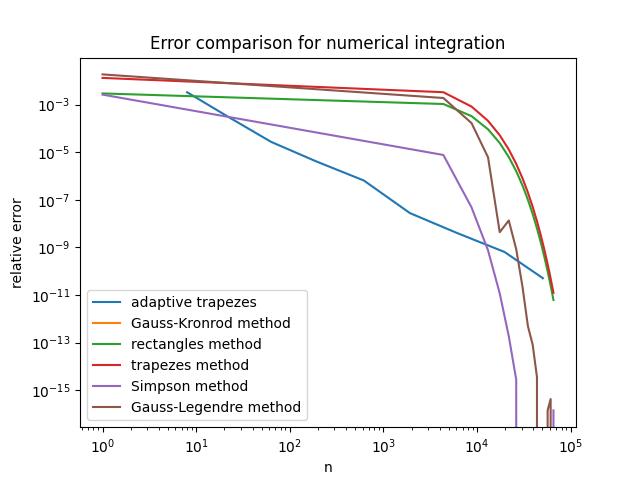
\includegraphics[width=0.8\linewidth]{integration2_1.png}
        \caption{Wartości błędu względnego dla różnych metod
        całkowania.}
    \end{figure}
    Najdokładniejszą metodą okazała się metoda adaptacyjna
    Gaussa-Kronroda, do tego stopnia, że w obliczeniach nie została
    zarejestrowana żadna wartość błędu. Drugą w kolejności jest metoda
    adaptacyjna trapezów. Pozostałe zachowywały się podobnie i miały
    nieco gorszą skuteczność.

    \subsection{Zadanie 2.}
    \begin{figure}[H]
        \centering
        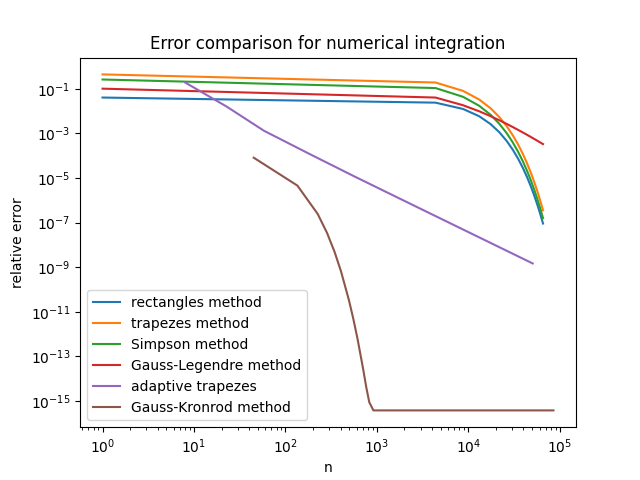
\includegraphics[width=0.7\linewidth]{integration2_2.png}
        \caption{Wartości błędu względnego dla różnych metod
            całkowania funkcji 1.}
    \end{figure}
    \begin{figure}[H]
        \centering
        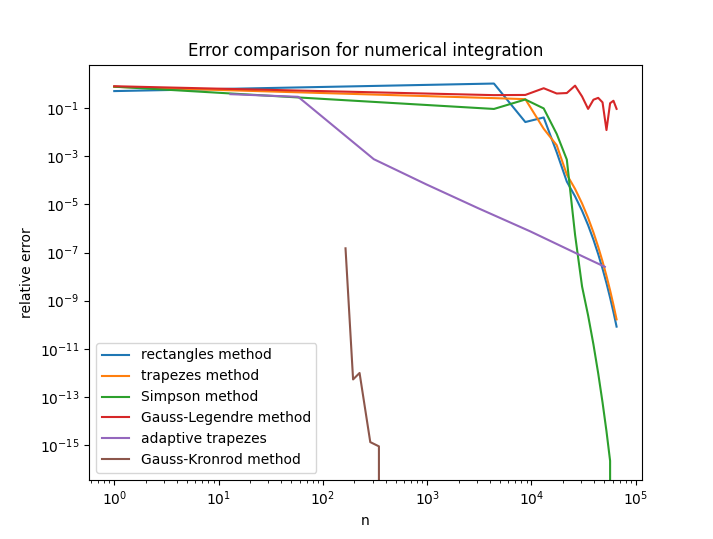
\includegraphics[width=0.7\linewidth]{integration2_3.png}
        \caption{Wartości błędu względnego dla różnych metod
            całkowania funkcji 2.}
    \end{figure}

    Dla obydwu całkowanych funkcji najdokładniejszą metodą ponownie
    okazała się metoda adaptacyjna Gaussa-Kronroda, a za nią, jednak
    już nie tak wysoce dokładna, metoda adaptacyjna trapezów.

    \section{Wnioski}
    Całkowanie numeryczne przy pomocy kwadratur adaptacyjnych jest
    znacznie dokładniejsze niż klasyczne kwadratury. Wynika to
    z odpowiedniego doboru punktów ewaluacji w przedziałach bardziej
    narażonych na zmienności funkcji. Dzięki temu można dokładnie
    oraz wydajnie obliczać całki nawet skomplikowanych funkcji. Jest
    to przydatne narzędzie obliczeniowe, jednak należy pamiętać, że
    każda metoda numeryczna może byc obarczona błędami.

    \section{Bibliografia}
    \url{https://en.wikipedia.org/wiki/Gauss\%E2\%80\%93
        Kronrod_quadrature_formula} \\
    \url{https://en.wikipedia.org/wiki/Adaptive_quadrature}

\end{document}
